\setcounter{framenumber}{0}
%25

\begin{frame}
  \titlepage
\end{frame}

\begin{frame}{Learning Goals}
By the end of this lecture, students should be able to:

\begin{itemize}
    \item interpret conditional probability intuitively;
    \item apply Bayes' rule and the Law of Total Probability;
    \item distinguish between $P(A|B)$ and $P(B|A)$;
    \item understand independence and conditional independence;
    \item use conditioning as a strategy in solving in probability problems.
\end{itemize}
\end{frame}

\lecturepart{Conditional Probability}
\begin{frame}{Why Do We Need Conditional Probability?}

In many situations, probabilities change once additional information becomes available.

\begin{columns}[T]

\column{0.48\textwidth}

\begin{block}{Before observing new information}
Let
\[
R=\{\text{it rains today}\}.
\]

Without any additional information, we assign the probability

\[
\Prob(R).
\]

This represents our initial uncertainty about rain.
\end{block}

\column{0.48\textwidth}

\begin{block}{After observing new information}
Suppose we now observe dark clouds:

\[
C=\{\text{dark clouds are present}\}.
\]

The probability of rain may now change to

\[
\Prob(R\mid C),
\]

read as $\text{``probability of }R\text{ given }C\text{.''}$.
\end{block}

\end{columns}

An important observation here is that we do not necessarily have $\Prob(R\mid C)= \Prob(R)$, because the information that $C$ occurred changes what outcomes now appear more plausible.

\begin{keybox}{Main Idea}
Conditional probability quantifies how probabilities are updated after new information or evidence is observed.
\end{keybox}

\end{frame}

\begin{frame}{Definition of Conditional Probability}
\begin{keybox}{Definition}
If
\[
\Prob(B)>0,
\]
then the conditional probability of $A$ given $B$ is

\[
\boxed{
\Prob(A|B)
=
\frac{\Prob(A\cap B)}{\Prob(B)}.
}
\]
\end{keybox}

\vspace{0.3cm}

Interpretation:
\begin{itemize}
    \item $B$ is the observed evidence;
    \item we restrict attention to outcomes in $B$;
    \item probabilities are renormalized within $B$.
\end{itemize}
\end{frame}


\begin{frame}{Visual Interpretation of Conditional Probability}

\begin{center}
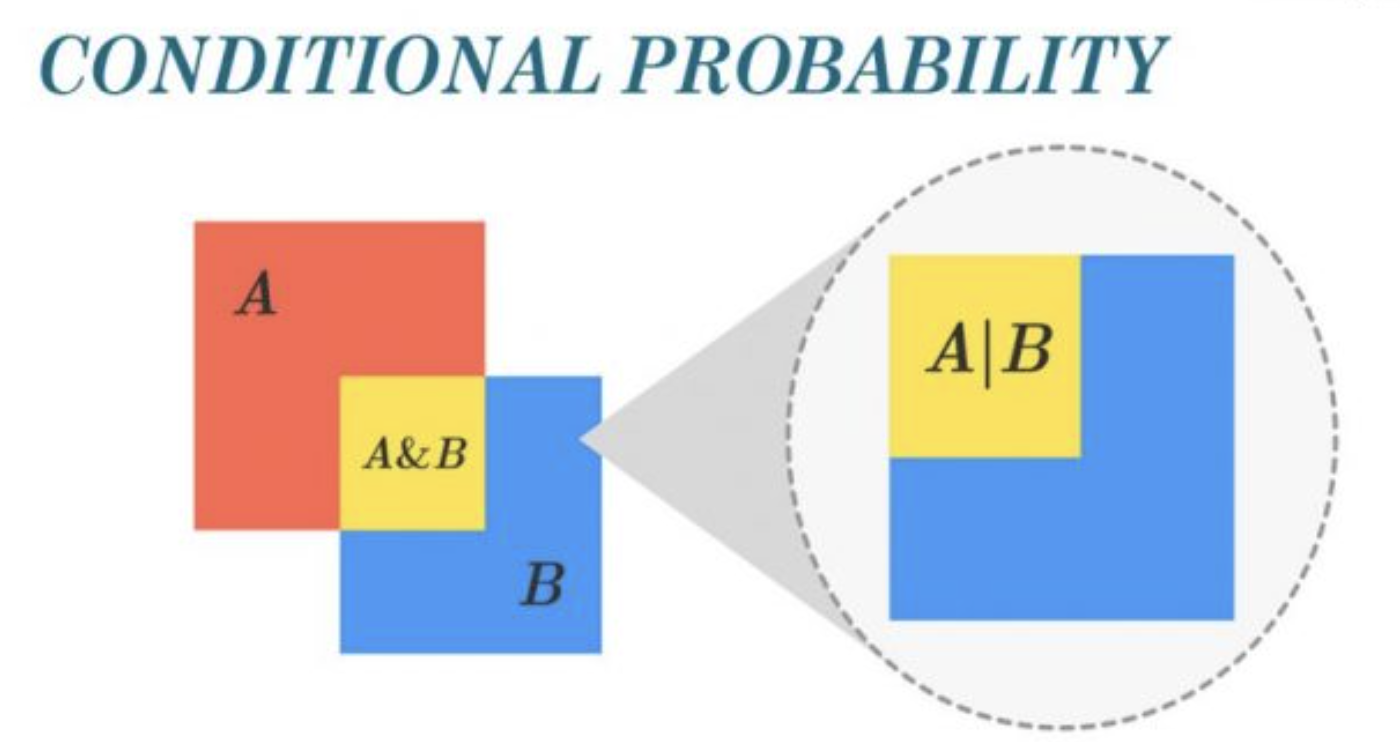
\includegraphics[width=0.49\textwidth]{assets/figures/cond.png}
\end{center}

\begin{center}
\small
When conditioning on $B$, the event $B$ becomes the new sample space (i.e., replaces $\Sample$).
The conditional probability $\Prob(A\mid B)$ measures the proportion of $B$
that also belongs to $A$.
\end{center}

\[
\boxed{
\Prob(A\mid B)=\frac{\Prob(A\cap B)}{\Prob(B)}
}
\qquad \text{provided } \Prob(B)>0.
\]

{\scriptsize
Image adapted from:
\href{https://www.excelr.com/blog/data-science/conditional-probability}
{ExcelR --- Conditional Probability}.
}

\end{frame}




\begin{frame}{Useful Equations from Conditional Probability}

\[
\Prob(A)
=
\Prob(A\mid B)\Prob(B)
+
\Prob(A\mid B^c)\Prob(B^c).
\]

\vspace{0.4cm}

\[
\Prob(B)
=
\Prob(B\mid A)\Prob(A)
+
\Prob(B\mid A^c)\Prob(A^c).
\]

\vspace{0.4cm}

\begin{keybox}{Law of Total Probability}
Each equation partitions the sample space into two disjoint cases and adds the corresponding conditional probabilities.
\end{keybox}

\end{frame}






\begin{frame}{Example: Two Cards}

Two cards are drawn without replacement.

Define
\[
A=\{\text{first card is a heart}\},
\qquad
B=\{\text{second card is red}\}.
\]

Using the multiplication rule,
\[
\Prob(A\cap B)
=
\Prob(B\mid A)\Prob(A)
=
\frac{25}{51}\cdot\frac{13}{52}
=
\frac{25}{204}.
\]

Also,
\[
\Prob(A)=\frac14,
\]
and
\[
\Prob(B)
=
\Prob(B\mid A)\Prob(A)
+
\Prob(B\mid A^c)\Prob(A^c)
=
\frac{25}{51}\cdot\frac14
+
\frac{17}{34}\cdot\frac34
=
\frac12.
\]

Therefore,
\[
\Prob(B\mid A)
=
\frac{\Prob(A\cap B)}{\Prob(A)}
=
\frac{25/204}{1/4}
=
\frac{25}{51}
\approx0.490,
\]
and
\[
\Prob(A\mid B)
=
\frac{\Prob(A\cap B)}{\Prob(B)}
=
\frac{25/204}{1/2}
=
\frac{25}{102}
\approx0.245.
\]

\end{frame}

\begin{frame}{Important Warning}
\begin{keybox}{Conditional probabilities are directional}
In general,

\[
\boxed{
\Prob(A|B)\neq\Prob(B|A).
}
\]
\end{keybox}

\vspace{0.25cm}

The conditioning event matters.

\vspace{0.25cm}

\[
\Prob(A|B)
\]

means:
\[
\text{probability of } A
\text{ after learning } B.
\]


\end{frame}

\lecturepart{Bayes' Rule and LOTP}

\begin{frame}{Intersection Formula}
From the definition:

\[
\Prob(A|B)
=
\frac{\Prob(A\cap B)}{\Prob(B)}.
\]

Multiplying both sides by $\Prob(B)$ gives:

\[
{
\Prob(A\cap B)
=
\Prob(B)\Prob(A|B).
}
\]

Similarly,

\[
\Prob(A\cap B)
=
\Prob(A)\Prob(B|A).
\]
The last two equalities together imply an important equality in Probability, known as the Bayes' rule, given in the next slide.
\end{frame}
\begin{frame}{Bayes' Rule: Updating Beliefs with Evidence}

\begin{keybox}{Bayes' Rule}
\[
\boxed{
\Prob(A\mid B)
=
\frac{\Prob(B\mid A)\Prob(A)}
{\Prob(B)}.
}
\]
\end{keybox}

Bayes' rule describes how probabilities "evolve" when new information is observed.

\begin{center}
\[
\underbrace{\Prob(A)}_{\text{before observing }B}
\quad
\Longrightarrow
\quad
\underbrace{\Prob(A\mid B)}_{\text{after observing }B}
=
\Prob(A)
\times
\underbrace{
\frac{\Prob(B\mid A)}{\Prob(B)}
}_{\text{updating weight}}
\]
\end{center}

The observation of $B$ changes our belief about whether $A$ occurred.

\begin{keybox}{Interpretation}
Bayes' rule updates a prior belief $\Prob(A)$ into a posterior belief $\Prob(A\mid B)$ by multiplying by a factor that measures how strongly the evidence $B$ supports $A$.
\end{keybox}

\end{frame}

\begin{frame}{Law of Total Probability}
Suppose
\[
A_1,\dots,A_n
\]
form a partition of $\Sample$.

Then:

\[
\boxed{
\Prob(B)
=
\sum_{i=1}^n
\Prob(B|A_i)\Prob(A_i).
}
\]

\vspace{0.25cm}

\begin{keybox}{Interpretation}
Break the sample space into cases, compute probabilities within each case, then combine them.
\end{keybox}
\end{frame}
\begin{frame}{Rare Disease Example}

Suppose we are analyzing the disease rate in a certain area. 

Let
\[
D=\{\text{person has the disease}\}, \quad T=\{\text{test result is positive}\},
\]
and assume

\[
\Prob(D)=0.01, \quad \Prob(T\mid D)=0.95, \quad  \Prob(T^c\mid D^c)=0.95.
\]


Interpretation:

\begin{itemize}
    \item The disease prevalence is $1\%$;
    \item The test correctly detects the disease $95\%$ of the time;
    \item The test correctly returns a negative result $95\%$ of the time for healthy individuals.
\end{itemize}

\vspace{0.2cm}

Question: A patient tests positive. What is $\Prob(D\mid T)?$

Using Bayes' Rule and the LOTP,

\[
\Prob(D\mid T)
=
\frac{\Prob(T\mid D)\Prob(D)}
{\Prob(T)} = \frac{\Prob(T\mid D)\Prob(D)}
{\Prob(T\mid D)\Prob(D)
+
\Prob(T\mid D^c)\Prob(D^c)} = \frac{0.95(0.01)}
{0.95(0.01)+0.05(0.99)}
\approx0.16.
\]
\end{frame}

\begin{frame}{Why This Feels Surprising}
Most people expect the answer to be close to $95\%$.

\vspace{0.25cm}

But the disease is very rare.

\vspace{0.25cm}

Among many healthy people:
\[
5\%
\]
still test positive.

\vspace{0.25cm}

Those false positives greatly outnumber the true positives.

\vspace{0.25cm}

\begin{keybox}{Lesson}
Posterior probabilities depend both on:
\begin{itemize}
    \item the evidence,
    \item and the prior probability.
\end{itemize}
\end{keybox}
\end{frame}

\lecturepart{Conditional Probability as Probability}
\begin{frame}{Conditional Probability is a Probability Measure}

Fix an event $E$ with
\[
\Prob(E)>0.
\]

Then the conditional probability function
\[
\Prob(\,\cdot\,\mid E)
\]
satisfies the three probability axioms.

\vspace{0.3cm}

\textbf{Axiom 1 (Nonnegativity)}
\[
\Prob(A\mid E)\ge 0
\qquad\text{for every event }A.
\]

\vspace{0.15cm}

\textbf{Axiom 2 (Normalization)}
\[
\Prob(\Sample\mid E)=1.
\]

\vspace{0.15cm}

\textbf{Axiom 3 (Countable Additivity)}
If $A_1,A_2,\ldots$ are pairwise disjoint events, then
\[
\Prob\!\left(\bigcup_{i=1}^{\infty}A_i\,\middle|\,E\right)
=
\sum_{i=1}^{\infty}\Prob(A_i\mid E).
\]

\end{frame}

\lecturepart{Independence}
\begin{frame}{Definition of Independence}

\begin{keybox}{Definition (Independence)}
Events $A$ and $B$ are independent if
\[
\Prob(A\mid B)=\Prob(A),
\]
provided $\Prob(B)>0$.
\end{keybox}


\textbf{Interpretation:}

Learning that $B$ occurred gives no information about $A$
(and vice versa$^\star$).


{\footnotesize
$(\star)$ We will later show that
\[
\Prob(A\mid B)=\Prob(A)
\quad\iff \quad
\Prob(B\mid A)=\Prob(B).
\]
Thus independence is symmetric:
\[
A \text{ is independent of } B
\iff
B \text{ is independent of } A.
\]
}

Think of it this way: $\mathbb{P}(A \text{ with new (additional) information}) = \mathbb{P}(A \ \text{with no additional information})$

\begin{keybox}{Lemma (Equivalent characterization of independence)}
Events $A$ and $B$ are independent if and only if
\[
\Prob(A\cap B)
=
\Prob(A)\times \Prob(B).
\]
\end{keybox}

\end{frame}

\begin{frame}{Conditional Independence}
\begin{keybox}{Conditional Independence}
Events $A$ and $B$ are conditionally independent given $E$ if

\[
\boxed{
\Prob(A\cap B|E)
=
\Prob(A|E)\Prob(B|E).
}
\]
\end{keybox}

\vspace{0.25cm}

Conditional independence is different from ordinary independence.

\vspace{0.25cm}

Two events may:
\begin{itemize}
    \item be independent but not conditionally independent;
    \item be conditionally independent but not independent.
\end{itemize}
\end{frame}
\begin{frame}{Example: A Hidden Variable Creates Dependence}

A coin is selected at random:

\begin{itemize}
    \item Fair coin with probability $1/2$;
    \item Biased coin ($P(H)=0.9$) with probability $1/2$.
\end{itemize}

\vspace{0.2cm}

\textbf{If we know which coin was selected:}

The tosses are independent.

\vspace{0.2cm}

\textbf{If we do not know which coin was selected:}

Observing early tosses changes our belief about which coin we have.

Therefore, earlier tosses affect our prediction of later tosses, so the tosses are \emph{not} independent.

\[
P(H_2\mid H_1)\neq P(H_2).
\]

\end{frame}

\lecturepart{Conditioning (Example)}



\begin{frame}{Monty Hall Problem: Setup}
\small

\begin{columns}[T]

\column{0.48\textwidth}

\begin{center}
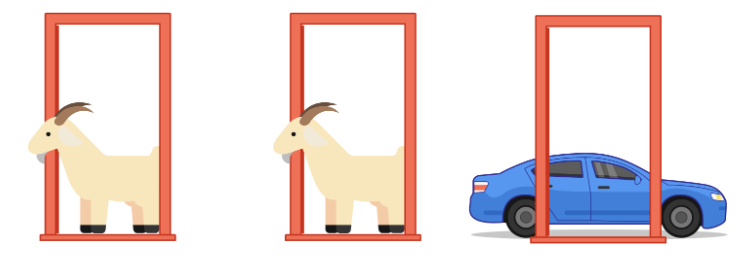
\includegraphics[width=\textwidth]{assets/figures/monty_all_doors.png}

{\scriptsize Image source: \href{https://brilliant.org/wiki/monty-hall-problem/}{Brilliant: Monty Hall Problem}.}
\end{center}

\column{0.52\textwidth}

There are three doors:

\begin{itemize}
    \item one door hides a car;
    \item two doors hide goats.
\end{itemize}

You choose one door, but it is not opened yet.

\vspace{0.2cm}

Assume, without loss of generality, that you initially choose door $1$.

\[
C_i=\{\text{car is behind door }i\}.
\]

Before Monty opens a door,

\[
\Prob(C_1)=\Prob(C_2)=\Prob(C_3)=\frac13.
\]

\end{columns}

\end{frame}







\begin{frame}{Monty Hall Problem: Why Switching Wins}
\small

\begin{columns}[T]

\column{0.42\textwidth}

\begin{center}
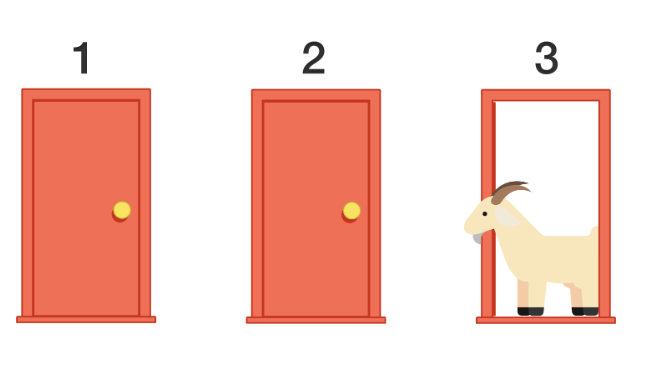
\includegraphics[width=\textwidth]{assets/figures/monty_one_goat_revealed.png}

{\scriptsize Image source: \href{https://brilliant.org/wiki/monty-hall-problem/}{Brilliant: Monty Hall Problem}.}
\end{center}

\column{0.58\textwidth}

Monty knows where the car is and always opens a door with a goat.

\vspace{0.15cm}

So the important question is:

\[
\text{Should you switch?}
\]

\[
\begin{array}{c|c|c}
\text{Car location} & \text{First choice} & \text{Switching} \\
\hline
C_1 & \text{correct} & \text{loses} \\
C_2 & \text{wrong} & \text{wins} \\
C_3 & \text{wrong} & \text{wins}
\end{array}
\]

\vspace{0.2cm}

Therefore,

\[
\Prob(\text{win by switching})
=
\Prob(C_2\cup C_3)
=
\Prob(C_2)+\Prob(C_3)
=
\frac13+\frac13
=
{\frac23}.
\]

\end{columns}

\end{frame}



\begin{frame}{Monty Hall Problem via Bayes' Rule}
    Suppose Monty opens door $3$.

Define
\[
M_3=\{\text{Monty opens door }3\}.
\]

Thus:

\[
\underbrace{\Prob(\text{initial choice correct})}_{\text{door }1}
=
\frac13, \quad \text{ and }  \quad \underbrace{\Prob(\text{initial choice wrong})}_{\text{door }2\text{ or }3}
=
\frac23.
\]



\vspace{0.2cm}

After Monty reveals a goat behind door $3$,
the entire remaining probability mass concentrates on door $2$.

Using Bayes' Rule,

\[
\Prob(\text{win by switching}|M_3) = \Prob(C_2\mid M_3)
=
\frac{\Prob(M_3\mid C_2)\Prob(C_2)}
{\Prob(M_3)}.
\]

Now, $\Prob(C_2)=\frac13,$ $\Prob(M_3\mid C_2)=1,$ and
\[
\Prob(M_3)
=
\frac12\cdot\frac13
+
1\cdot\frac13
+
0\cdot\frac13
=
\frac12.
\]

Therefore,

\[
\Prob(C_2\mid M_3)
=
\frac{1\cdot\frac13}{\frac12}
=
{\frac23}, \text{ and thus}\ \ \text{, and thus } \ \Prob(\text{win without switching} | M_3) = \mathbb{P}(C_1|M_3) = \frac{1}{3}
\]
Hence, switching doors wins with probability

\end{frame}

\begin{frame}{Summary}
\begin{itemize}
    \item Conditional probability updates probabilities using observed evidence.

    \item
    \[
    \Prob(A|B)
    =
    \frac{\Prob(A\cap B)}{\Prob(B)}.
    \]

    \item Bayes' Rule relates:
    \[
    \Prob(A|B)
    \quad \text{and} \quad
    \Prob(B|A).
    \]

    \item LOTP breaks problems into cases.

    \item Conditional probabilities themselves satisfy the probability axioms.

    \item Independence means:
    \[
    \Prob(A|B)=\Prob(A).
    \]

    \item Conditioning is a powerful problem-solving strategy.
\end{itemize}

\vspace{0.25cm}

\begin{keybox}{Next lecture}
Random variables and distributions.
\end{keybox}
\end{frame}